\documentclass[11pt,a4paper]{article}
\usepackage[T1]{fontenc}
\usepackage[utf8]{inputenc}
\usepackage[margin=1in]{geometry}
\usepackage{graphicx}
\usepackage{subcaption}
\usepackage{booktabs}
\usepackage{array}
\usepackage{float}
\usepackage{parskip}
\usepackage[hidelinks]{hyperref}

\title{Report on the Aachen Old Pain2D Dataset}
\author{Raj Singh}
\date{\today}

\begin{document}
\maketitle

\section{Dataset Summary}

The four-class version of the Aachen old dataset contains the following categories:

\begin{table}[H]
    \centering
    \begin{tabular}{|c|l|c|c|}
        \toprule
        & \textbf{Class} & \textbf{Images} & \textbf{Role in Report} \\
        \midrule
        1 & EDS old & 60 & Included in 4-class task \\
        2 & FSHD & 35 & Included in 4-class task \\
        3 & GBS & 32 & Included in 4-class task \\
        4 & PROMM & 90 & Included in 4-class task \\
        \midrule
        & Total & 217 & Full old Aachen cohort used here \\
        \bottomrule
    \end{tabular}
    \caption{Class composition of the Aachen old Pain2D dataset.}
\end{table}

For the four-class experiment, class balancing by undersampling produced an effective training pool of 32 samples per class. In addition, a reduced binary task was evaluated separately. The exact binary class pair is part of the reduced experimental setup, while the current report focuses mainly on the observed performance and model comparison.

\section{Experimental Design}

Two main experiment families were carried out on this dataset:

\begin{itemize}
    \item a reduced 2-class experiment, evaluated with \textit{FCNNNet}, \textit{FCNNSmall}, and \textit{SimpleCNNSmall},
    \item a 4-class experiment, evaluated with \textit{FCNNNet}.
\end{itemize}

All experiments used the same general training pipeline: grayscale conversion, image resizing, saved tensor generation, balanced sampling through undersampling, and standard train-validation splitting.

\begin{table}[H]
    \centering
    \begin{tabular}{|c|l|c|c|c|}
        \toprule
        & \textbf{Task} & \textbf{Model} & \textbf{Train Accuracy (\%) (max)} & \textbf{Validation Accuracy (\%) (max)} \\
        \midrule
        1 & 2-class & FCNNNet & 100.00 & 100.00 \\
        2 & 2-class & FCNNSmall & 84.44 & 100.00 \\
        3 & 2-class & SimpleCNNSmall & 100.00 & 100.00 \\
        4 & 4-class & FCNNNet & 100.00 & 90.38 \\
        \bottomrule
    \end{tabular}
    \caption{Final train and validation accuracy achieved by each reported model on the Aachen old dataset.}
\end{table}

\section{Results}

\subsection{Binary Task}

The binary (i.e., EDS old and PROMM) Aachen-old experiment produced an unusually strong and clean result. All three tested models reached a perfect normalized confusion matrix on the validation split, with diagonal values of 1.00 and off-diagonal values of 0.00. This means that, for the selected binary subset, every model separated the two classes perfectly in the reported run.

This is an important result for the project because it suggests that the underlying signal in the Aachen old dataset is much clearer than in several other cohorts studied so far. When three different architectures all converge to the same perfect class separation, this is a strong indication that the dataset is internally consistent and visually informative.

\begin{figure}[H]
    \centering
    \begin{subfigure}{0.32\textwidth}
        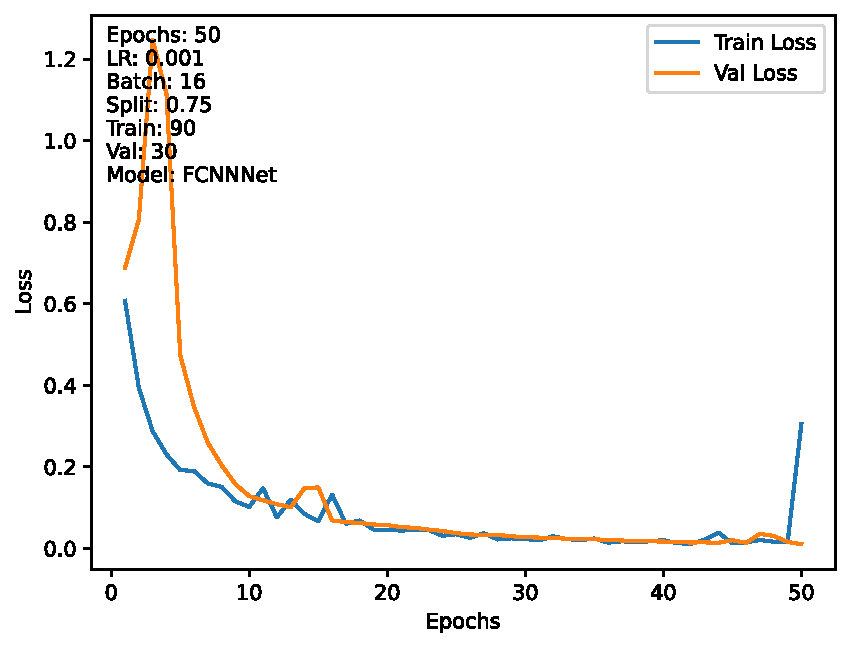
\includegraphics[width=\linewidth]{images/aachen_old_dataset_num_classes_2_FCNNNet_loss.pdf}
        \caption{FCNNNet - Loss}
    \end{subfigure}
    \hfill
    \begin{subfigure}{0.32\textwidth}
        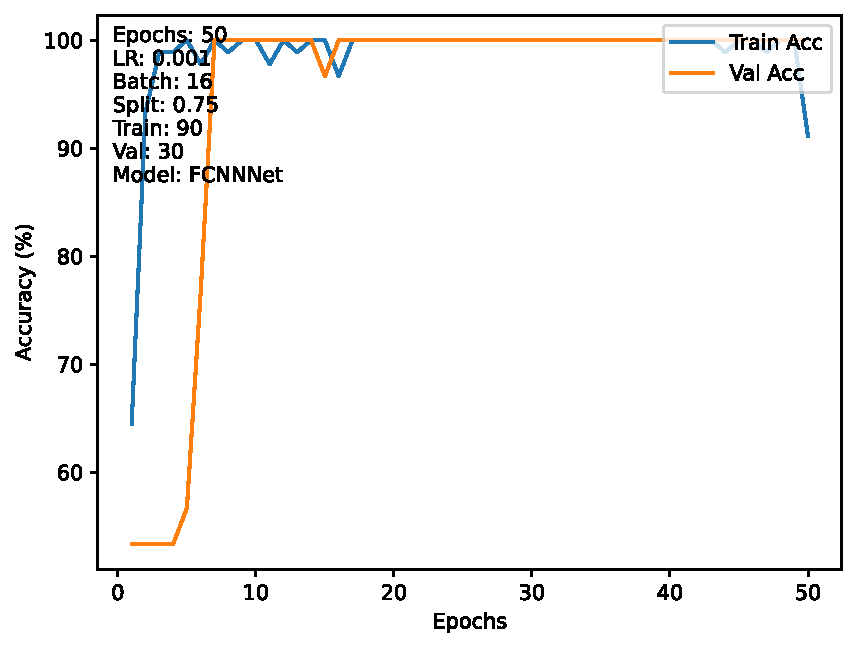
\includegraphics[width=\linewidth]{images/aachen_old_dataset_num_classes_2_FCNNNet_accuracy.pdf}
        \caption{FCNNNet - Accuracy}
    \end{subfigure}
    \hfill
    \begin{subfigure}{0.32\textwidth}
        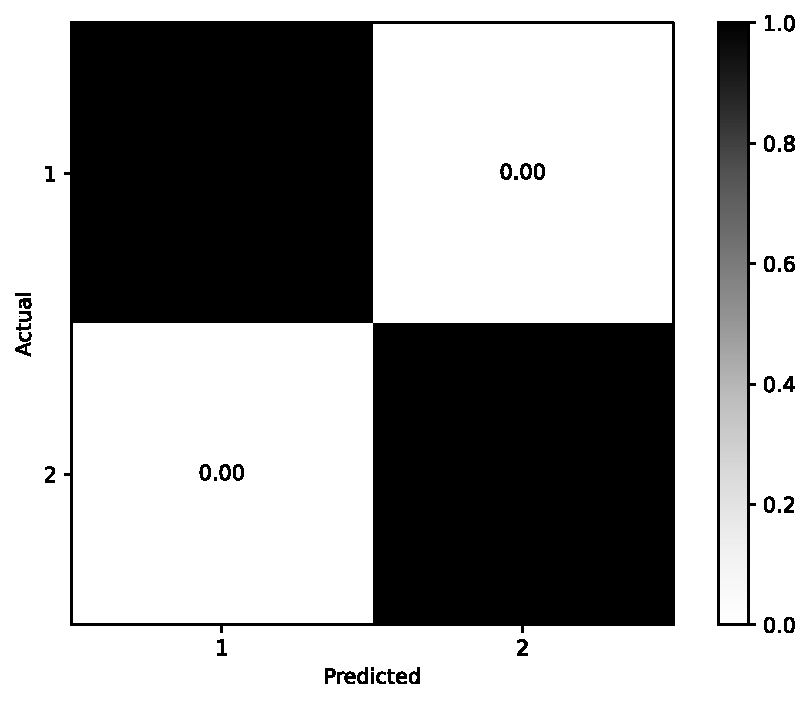
\includegraphics[width=\linewidth]{images/aachen_old_dataset_num_classes_2_FCNNNet_confusion_matrix.pdf}
        \caption{FCNNNet - Confusion Matrix}
    \end{subfigure}

    \vspace{0.3cm}

    \begin{subfigure}{0.32\textwidth}
        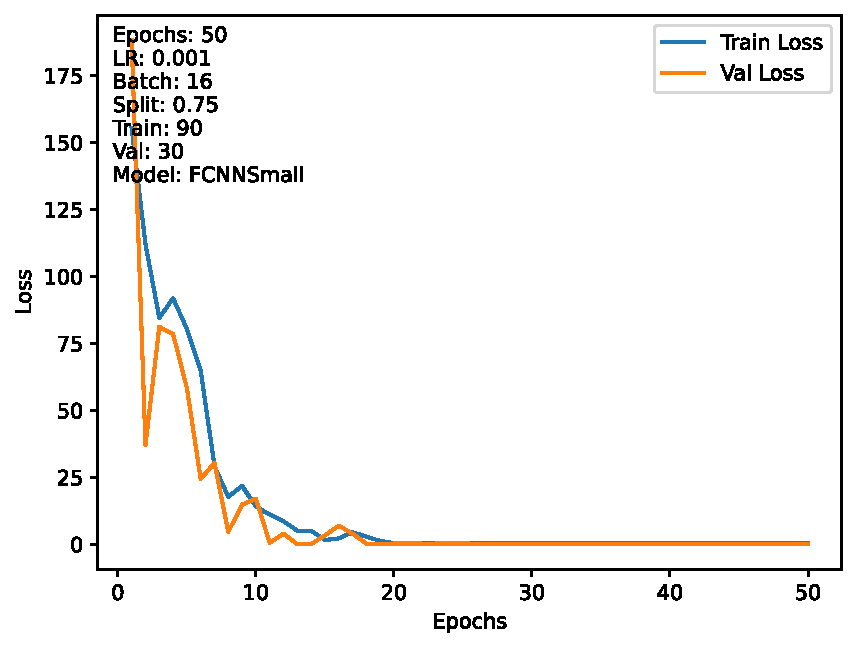
\includegraphics[width=\linewidth]{images/aachen_old_dataset_num_classes_2_FCNNSmall_loss.pdf}
        \caption{FCNNSmall - Loss}
    \end{subfigure}
    \hfill
    \begin{subfigure}{0.32\textwidth}
        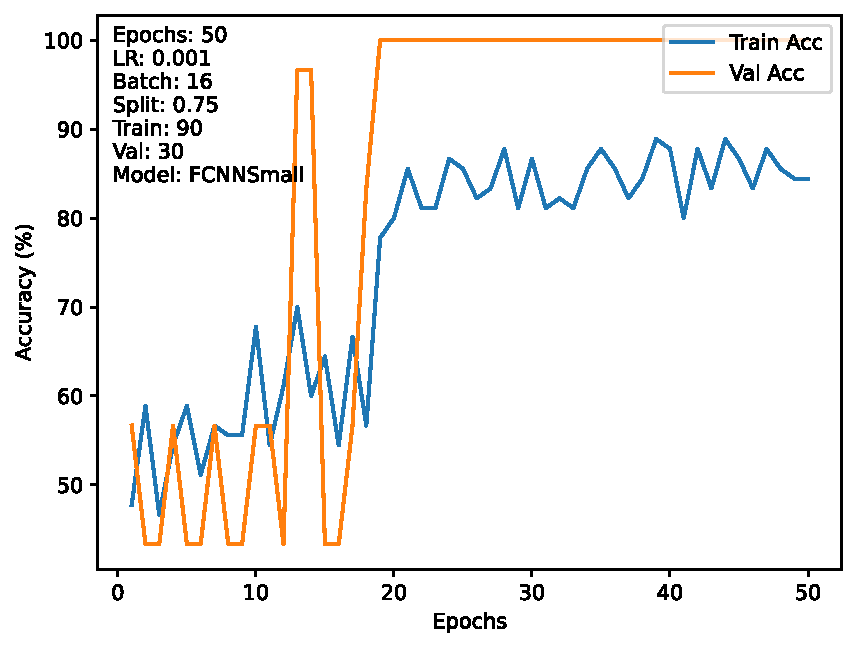
\includegraphics[width=\linewidth]{images/aachen_old_dataset_num_classes_2_FCNNSmall_accuracy.pdf}
        \caption{FCNNSmall - Accuracy}
    \end{subfigure}
    \hfill
    \begin{subfigure}{0.32\textwidth}
        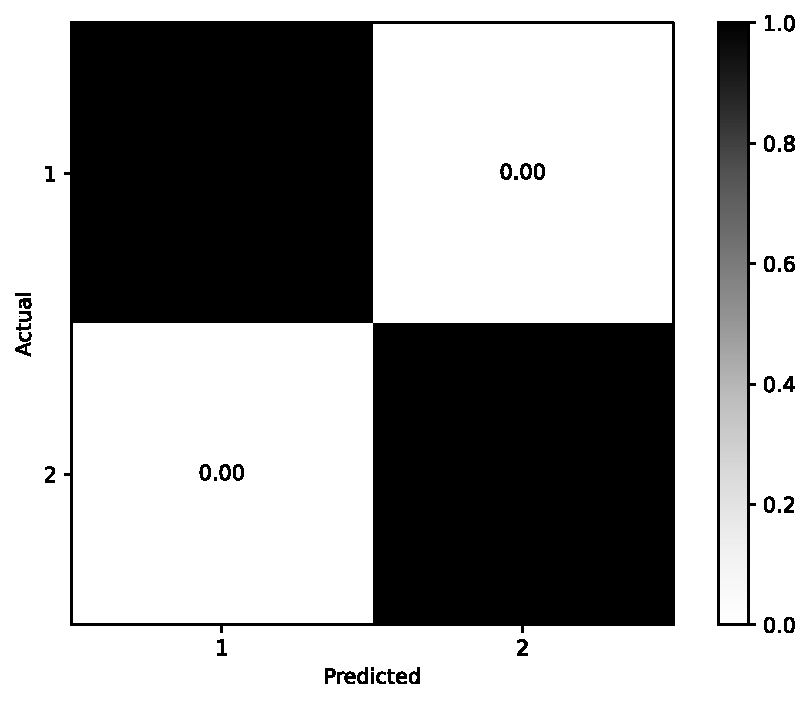
\includegraphics[width=\linewidth]{images/aachen_old_dataset_num_classes_2_FCNNSmall_confusion_matrix.pdf}
        \caption{FCNNSmall - Confusion Matrix}
    \end{subfigure}

    \vspace{0.3cm}

    \begin{subfigure}{0.32\textwidth}
        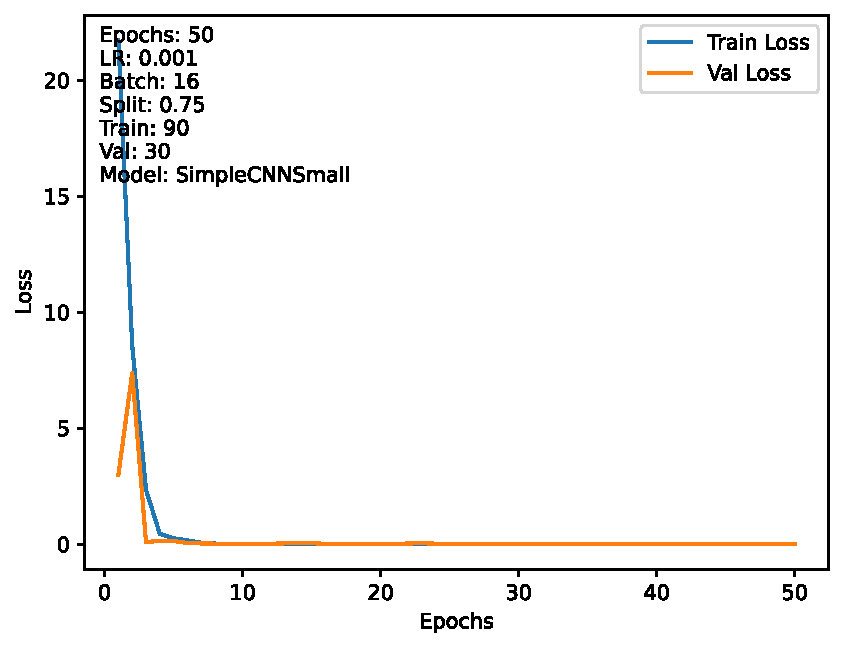
\includegraphics[width=\linewidth]{images/aachen_old_dataset_num_classes_2_SimpleCNNSmall_loss.pdf}
        \caption{SimpleCNNSmall - Loss}
    \end{subfigure}
    \hfill
    \begin{subfigure}{0.32\textwidth}
        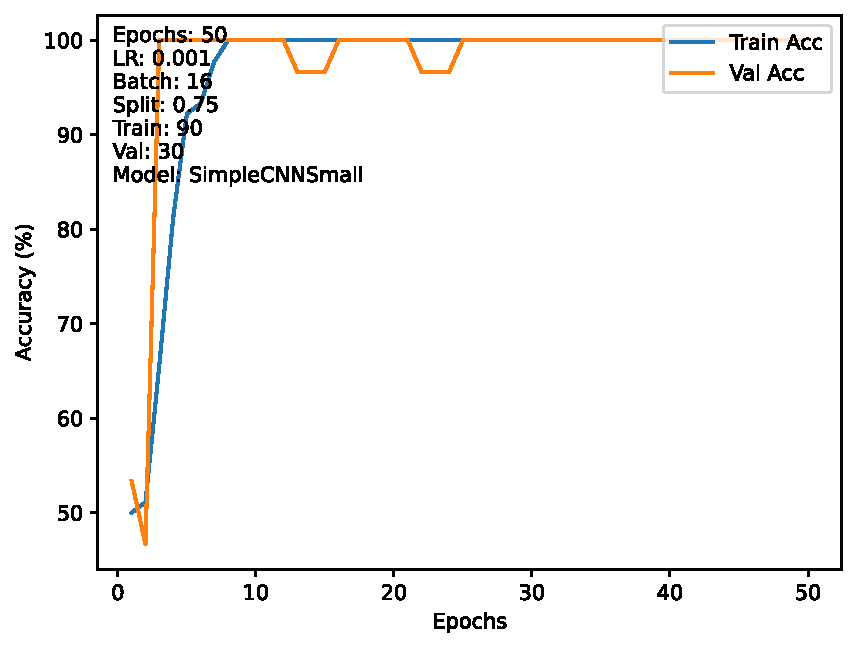
\includegraphics[width=\linewidth]{images/aachen_old_dataset_num_classes_2_SimpleCNNSmall_accuracy.pdf}
        \caption{SimpleCNNSmall - Accuracy}
    \end{subfigure}
    \hfill
    \begin{subfigure}{0.32\textwidth}
        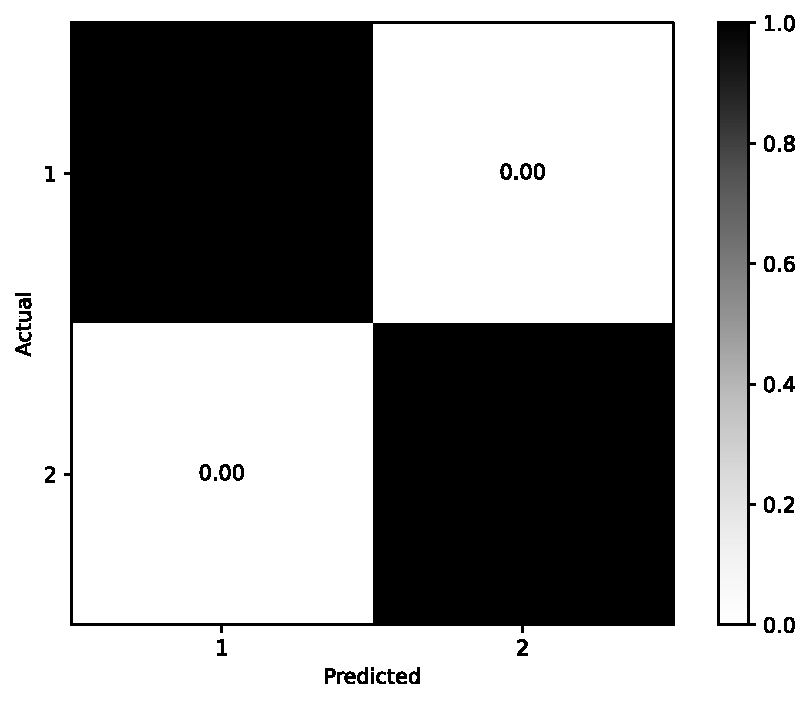
\includegraphics[width=\linewidth]{images/aachen_old_dataset_num_classes_2_SimpleCNNSmall_confusion_matrix.pdf}
        \caption{SimpleCNNSmall - Confusion Matrix}
    \end{subfigure}

    \caption{Binary classification results on the Aachen old dataset. All three models achieved perfect separation in the reported run.}
\end{figure}

\subsection{Four-Class Task}

The most important multi-class result was obtained with \textit{FCNNNet} on the 4-class task. In the strongest run, which used the cropping-based preprocessing step, the row-normalized confusion matrix shows consistently high recall across all four diagnostic groups:

\begin{itemize}
    \item EDS old: 0.90
    \item FSHD: 0.75
    \item GBS: 0.89
    \item PROMM: 0.80
\end{itemize}

These values are very encouraging for a four-class pain-drawing classification problem. The result is especially important because all four classes remain clinically distinct and visually nontrivial, yet the model still preserves strong recall in every group. In practical terms, this is one of the clearest signs in the current project that high-quality acquisition and high-quality scanning can translate directly into better machine-learning performance.

The cropped preprocessing variant also appears to have improved the class balance of the predictions. In an earlier non-cropped four-class run, the model still showed much stronger confusion between some categories, especially for PROMM. After cropping-based preprocessing, the confusion matrix became much more balanced, which suggests that removing non-informative image regions helped the network focus on the clinically relevant spatial signal.

\begin{figure}[H]
    \centering
    \begin{subfigure}{0.32\textwidth}
        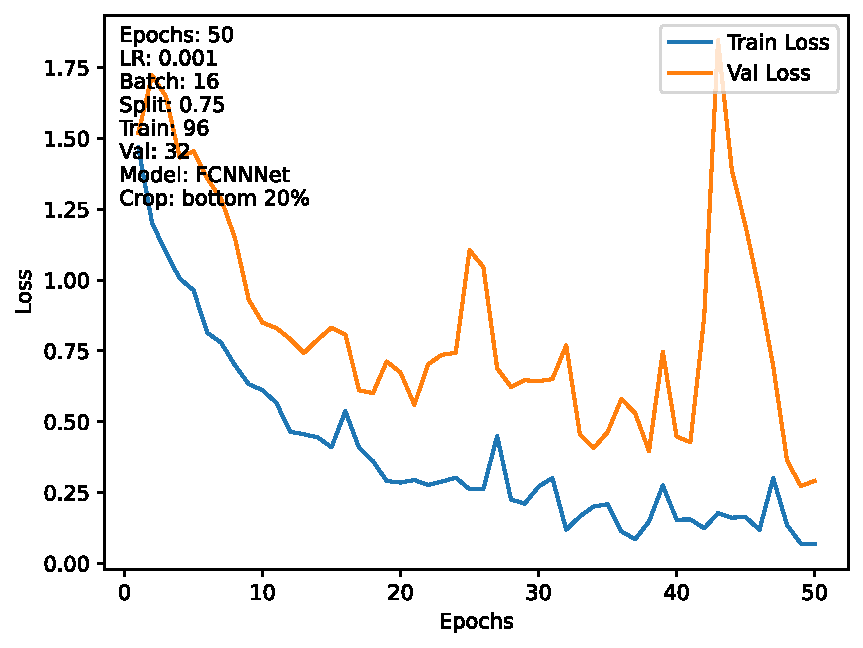
\includegraphics[width=\linewidth]{images/aachen_old_dataset_cropped_num_classes_4_FCNNNet_loss.pdf}
        \caption{Loss}
    \end{subfigure}
    \hfill
    \begin{subfigure}{0.32\textwidth}
        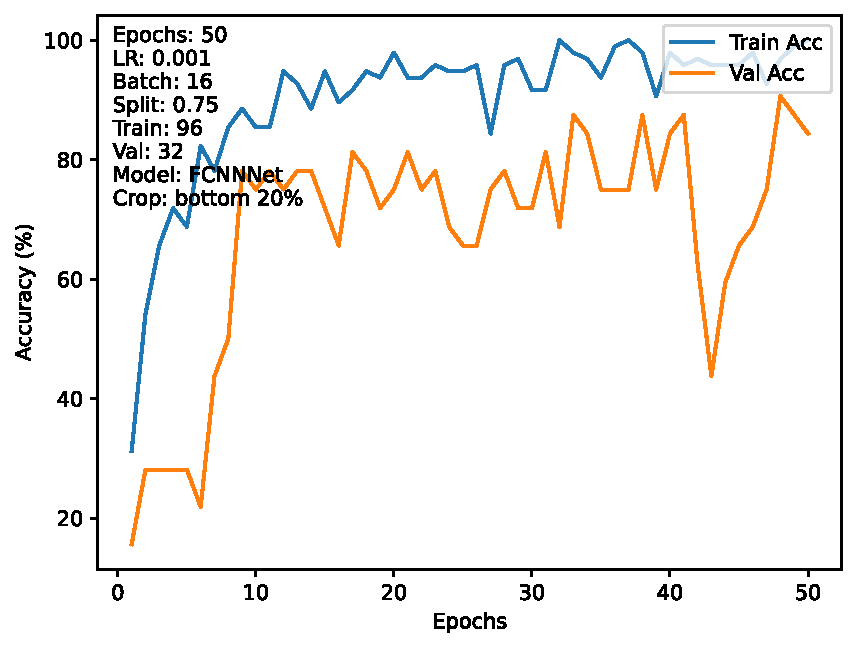
\includegraphics[width=\linewidth]{images/aachen_old_dataset_cropped_num_classes_4_FCNNNet_accuracy.pdf}
        \caption{Accuracy}
    \end{subfigure}
    \hfill
    \begin{subfigure}{0.32\textwidth}
        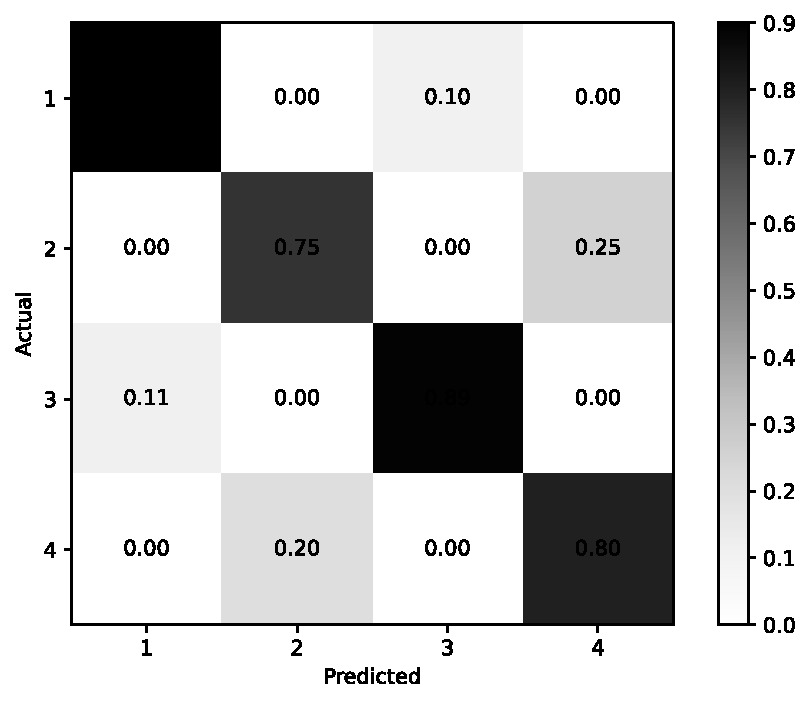
\includegraphics[width=\linewidth]{images/aachen_old_dataset_cropped_num_classes_4_FCNNNet_confusion_matrix.pdf}
        \caption{Confusion Matrix}
    \end{subfigure}
    \caption{Best reported 4-class result on the Aachen old dataset using FCNNNet.}
\end{figure}

\section{Interpretation}

The Aachen old dataset stands out because the experimental behavior is not merely acceptable, but unusually strong. The binary task is perfectly separated by all tested models, and the four-class task reaches high recall across all categories in the best run.

Therefore, the current evidence supports the following interpretation:

\begin{itemize}
    \item the Aachen old dataset was acquired with a relatively high level of care,
    \item the scans appear to be clean, well aligned, and visually stable,
    \item the dataset contains a stronger disease-related signal than several other currently available cohorts in the project.
\end{itemize}

\section{Conclusion}

The Aachen old Pain2D dataset delivered very strong results in the recent experiments. The reduced binary task was solved perfectly by all three tested models, while the four-class \textit{FCNNNet} experiment achieved high recall across all four classes. Taken together, these results strongly suggest that the dataset is both clinically informative and technically well acquired.

This makes the Aachen old dataset one of the most promising datasets in the current project. It is a strong example of how careful acquisition and good scanning quality can materially improve downstream machine-learning performance on pain drawings.

\end{document}
